\documentclass{standalone}
\usepackage{tikz}
\usetikzlibrary{patterns, positioning}
\usepackage[sfdefault]{ClearSans} %% option 'sfdefault' activates Clear Sans as the default text font
\usepackage[T1]{fontenc}

\begin{document}
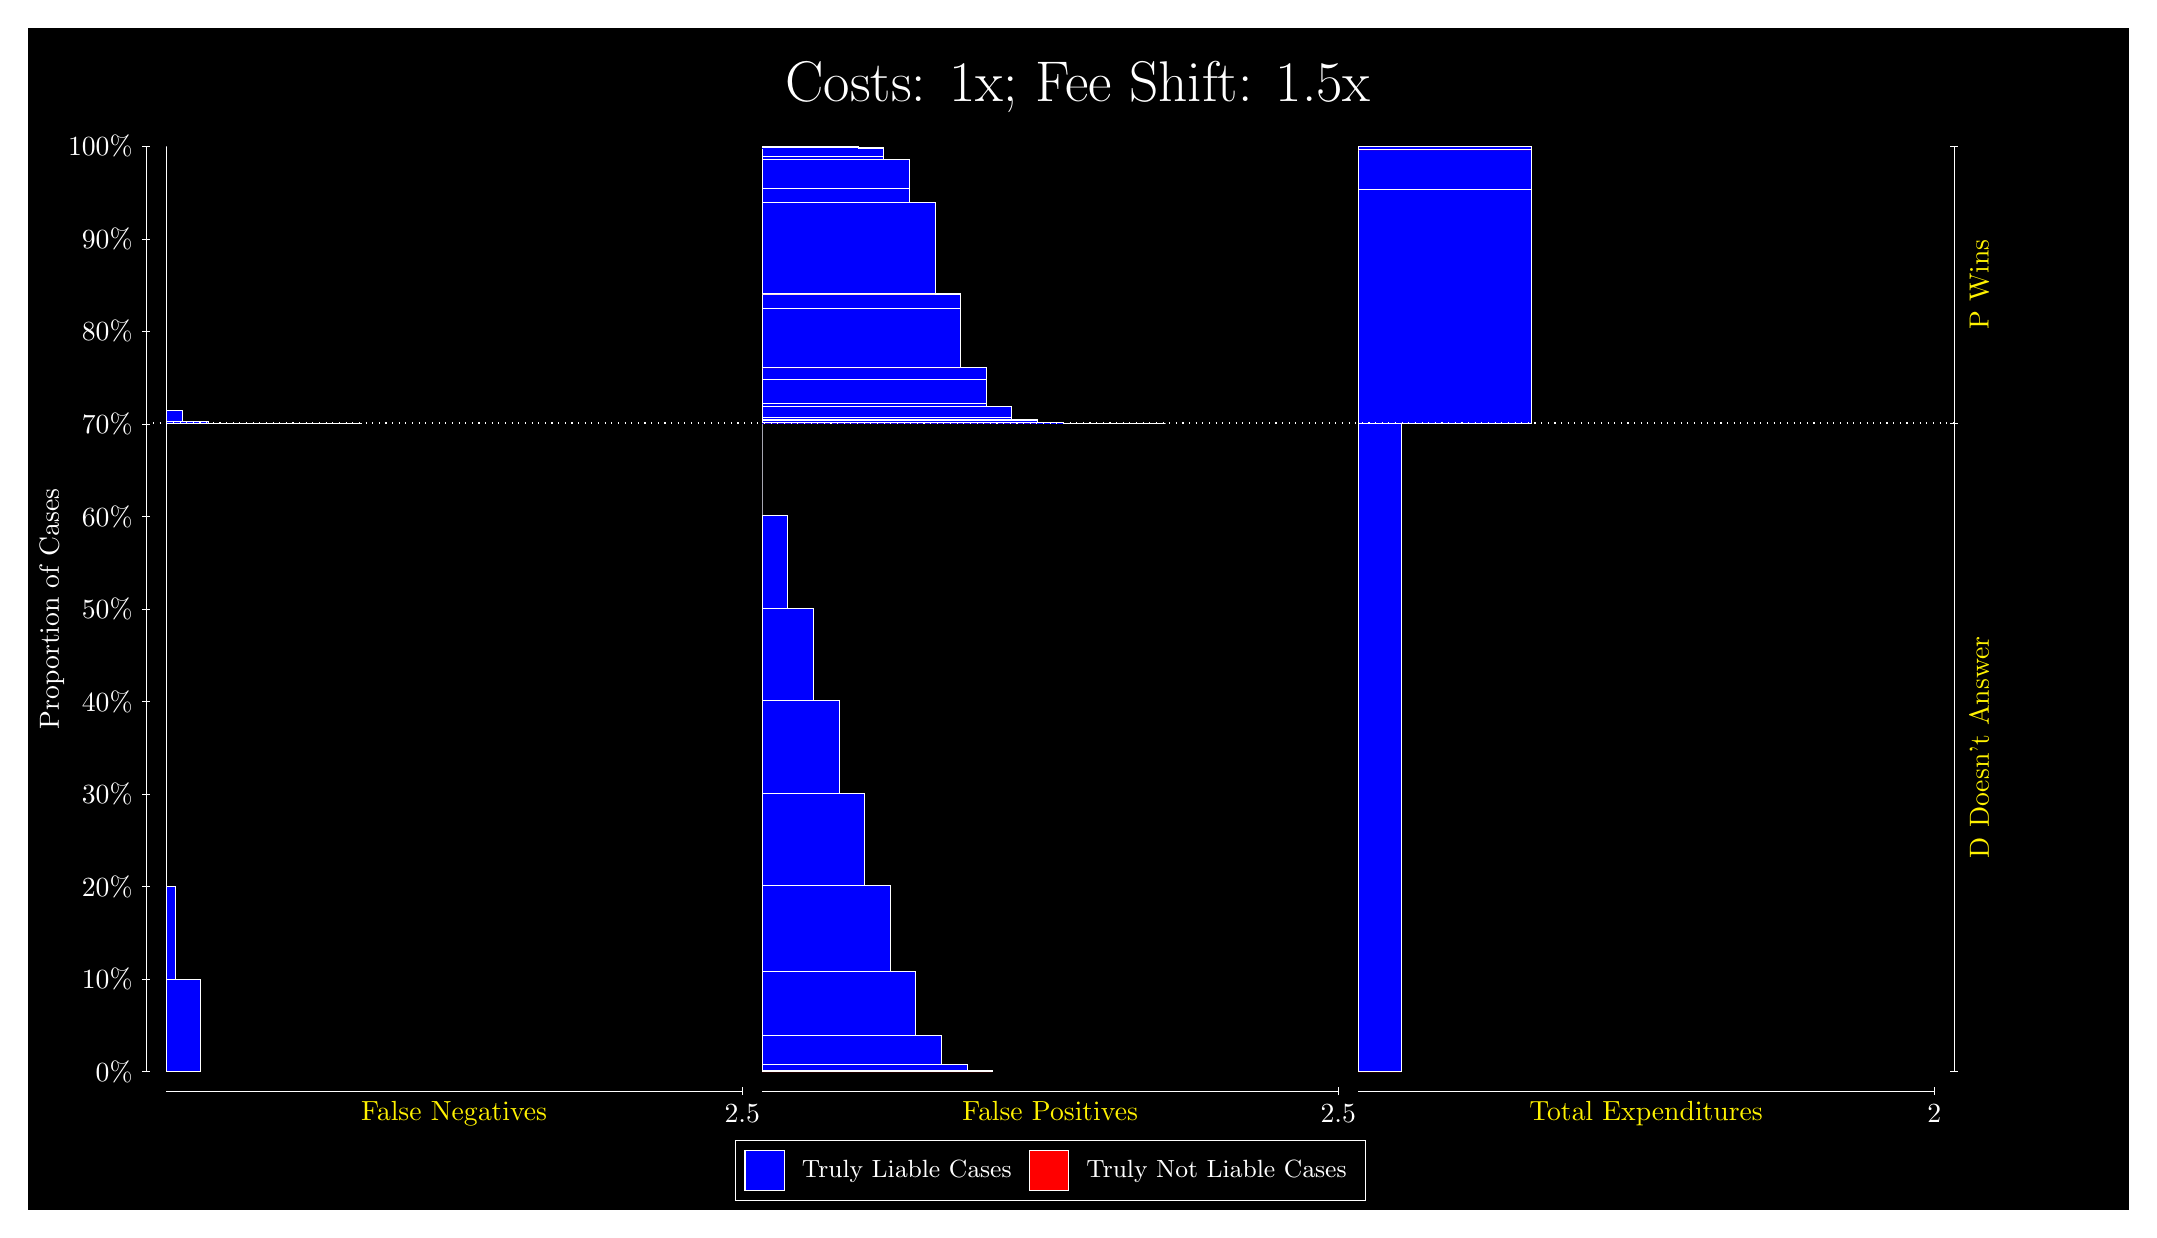
\begin{tikzpicture}
\draw[fill=black] (0,0) rectangle (26.667,15);
\draw[text=white] (0,13.5) rectangle (26.667,15) node[midway] {\huge Costs: 1x; Fee Shift: 1.5x};
\draw[white, very thin] (1.5,1.75) -- (1.5,13.5);
\node[rotate=90, text=white, anchor=center] at (0.3, 7.625) {Proportion of Cases};
\draw[white, very thin] (1.45,1.75) -- (1.55,1.75);
\node[text=white, anchor=east] at (1.45, 1.75) {0\%};
\draw[white, very thin] (1.45,2.925) -- (1.55,2.925);
\node[text=white, anchor=east] at (1.45, 2.925) {10\%};
\draw[white, very thin] (1.45,4.1) -- (1.55,4.1);
\node[text=white, anchor=east] at (1.45, 4.1) {20\%};
\draw[white, very thin] (1.45,5.275) -- (1.55,5.275);
\node[text=white, anchor=east] at (1.45, 5.275) {30\%};
\draw[white, very thin] (1.45,6.45) -- (1.55,6.45);
\node[text=white, anchor=east] at (1.45, 6.45) {40\%};
\draw[white, very thin] (1.45,7.625) -- (1.55,7.625);
\node[text=white, anchor=east] at (1.45, 7.625) {50\%};
\draw[white, very thin] (1.45,8.8) -- (1.55,8.8);
\node[text=white, anchor=east] at (1.45, 8.8) {60\%};
\draw[white, very thin] (1.45,9.975) -- (1.55,9.975);
\node[text=white, anchor=east] at (1.45, 9.975) {70\%};
\draw[white, very thin] (1.45,11.15) -- (1.55,11.15);
\node[text=white, anchor=east] at (1.45, 11.15) {80\%};
\draw[white, very thin] (1.45,12.325) -- (1.55,12.325);
\node[text=white, anchor=east] at (1.45, 12.325) {90\%};
\draw[white, very thin] (1.45,13.5) -- (1.55,13.5);
\node[text=white, anchor=east] at (1.45, 13.5) {100\%};

\draw[white, very thin] (24.457,1.75) -- (24.457,13.5);
\draw[white, very thin] (24.407,1.75) -- (24.507,1.75);
\node[anchor=west] at (24.407, 1.75) {};
\draw[white, very thin] (24.407,9.9861) -- (24.507,9.9861);
\node[anchor=west] at (24.407, 9.9861) {};
\draw[white, very thin] (24.407,13.5) -- (24.507,13.5);
\node[anchor=west] at (24.407, 13.5) {};

\draw[white, very thin, fill=blue] (1.75,1.75) rectangle (2.1891,2.925);
\draw[white, very thin, fill=blue] (1.75,2.925) rectangle (1.8638,4.1);
\draw[white, very thin, fill=red] (1.75,4.1) rectangle (1.75,4.1);
\draw[white, very thin, fill=blue] (1.75,4.1) rectangle (1.75,9.9861);
\draw[white, very thin, fill=blue] (1.75,9.9861) rectangle (4.2384,9.9861);
\draw[white, very thin, fill=blue] (1.75,9.9861) rectangle (3.9131,9.9861);
\draw[white, very thin, fill=blue] (1.75,9.9861) rectangle (3.5878,9.9861);
\draw[white, very thin, fill=blue] (1.75,9.9861) rectangle (3.2626,9.9861);
\draw[white, very thin, fill=blue] (1.75,9.9861) rectangle (3.2626,9.9861);
\draw[white, very thin, fill=blue] (1.75,9.9861) rectangle (2.9373,9.9861);
\draw[white, very thin, fill=blue] (1.75,9.9861) rectangle (2.9373,9.9861);
\draw[white, very thin, fill=blue] (1.75,9.9861) rectangle (2.9373,9.9861);
\draw[white, very thin, fill=blue] (1.75,9.9861) rectangle (2.612,9.9861);
\draw[white, very thin, fill=blue] (1.75,9.9861) rectangle (2.612,9.9868);
\draw[white, very thin, fill=blue] (1.75,9.9868) rectangle (2.2867,9.9868);
\draw[white, very thin, fill=blue] (1.75,9.9868) rectangle (2.2867,9.9871);
\draw[white, very thin, fill=blue] (1.75,9.9871) rectangle (2.2867,10.004);
\draw[white, very thin, fill=blue] (1.75,10.004) rectangle (1.9614,10.005);
\draw[white, very thin, fill=blue] (1.75,10.005) rectangle (1.9614,10.148);
\draw[white, very thin, fill=blue] (1.75,10.148) rectangle (1.9614,10.148);
\draw[white, very thin, fill=red] (1.75,10.148) rectangle (1.75,10.148);
\draw[white, very thin, fill=blue] (1.75,10.148) rectangle (1.75,13.5);
\draw[white, very thin, fill=red] (9.3189,1.75) rectangle (12.246,1.75);
\draw[white, very thin, fill=blue] (9.3189,1.75) rectangle (12.246,1.7606);
\draw[white, very thin, fill=blue] (9.3189,1.7606) rectangle (11.921,1.8447);
\draw[white, very thin, fill=blue] (9.3189,1.8447) rectangle (11.596,2.2095);
\draw[white, very thin, fill=blue] (9.3189,2.2095) rectangle (11.271,3.0221);
\draw[white, very thin, fill=blue] (9.3189,3.0221) rectangle (10.945,4.1186);
\draw[white, very thin, fill=blue] (9.3189,4.1186) rectangle (10.62,5.2863);
\draw[white, very thin, fill=blue] (9.3189,5.2863) rectangle (10.295,6.461);
\draw[white, very thin, fill=blue] (9.3189,6.461) rectangle (9.9694,7.636);
\draw[white, very thin, fill=blue] (9.3189,7.636) rectangle (9.6442,8.8111);
\draw[white, very thin, fill=blue] (9.3189,8.8111) rectangle (9.3189,9.9861);
\draw[white, very thin, fill=red] (9.3189,9.9861) rectangle (14.442,9.9861);
\draw[white, very thin, fill=blue] (9.3189,9.9861) rectangle (14.442,9.9861);
\draw[white, very thin, fill=red] (9.3189,9.9861) rectangle (14.117,9.9861);
\draw[white, very thin, fill=blue] (9.3189,9.9861) rectangle (14.117,9.9861);
\draw[white, very thin, fill=red] (9.3189,9.9861) rectangle (13.792,9.9861);
\draw[white, very thin, fill=blue] (9.3189,9.9861) rectangle (13.792,9.9861);
\draw[white, very thin, fill=blue] (9.3189,9.9861) rectangle (13.466,9.9861);
\draw[white, very thin, fill=red] (9.3189,9.9861) rectangle (13.466,9.9861);
\draw[white, very thin, fill=blue] (9.3189,9.9861) rectangle (13.466,9.9866);
\draw[white, very thin, fill=red] (9.3189,9.9866) rectangle (13.141,9.9866);
\draw[white, very thin, fill=blue] (9.3189,9.9866) rectangle (13.141,9.9894);
\draw[white, very thin, fill=blue] (9.3189,9.9894) rectangle (13.141,9.9921);
\draw[white, very thin, fill=red] (9.3189,9.9921) rectangle (12.816,9.9921);
\draw[white, very thin, fill=blue] (9.3189,9.9921) rectangle (12.816,10.022);
\draw[white, very thin, fill=blue] (9.3189,10.022) rectangle (12.816,10.03);
\draw[white, very thin, fill=blue] (9.3189,10.03) rectangle (12.49,10.062);
\draw[white, very thin, fill=red] (9.3189,10.062) rectangle (12.49,10.062);
\draw[white, very thin, fill=blue] (9.3189,10.062) rectangle (12.49,10.199);
\draw[white, very thin, fill=blue] (9.3189,10.199) rectangle (12.165,10.239);
\draw[white, very thin, fill=red] (9.3189,10.239) rectangle (12.165,10.239);
\draw[white, very thin, fill=blue] (9.3189,10.239) rectangle (12.165,10.538);
\draw[white, very thin, fill=blue] (9.3189,10.538) rectangle (12.165,10.691);
\draw[white, very thin, fill=red] (9.3189,10.691) rectangle (11.84,10.691);
\draw[white, very thin, fill=blue] (9.3189,10.691) rectangle (11.84,11.448);
\draw[white, very thin, fill=blue] (9.3189,11.448) rectangle (11.84,11.627);
\draw[white, very thin, fill=blue] (9.3189,11.627) rectangle (11.84,11.629);
\draw[white, very thin, fill=red] (9.3189,11.629) rectangle (11.515,11.629);
\draw[white, very thin, fill=blue] (9.3189,11.629) rectangle (11.515,12.79);
\draw[white, very thin, fill=blue] (9.3189,12.79) rectangle (11.515,12.79);
\draw[white, very thin, fill=blue] (9.3189,12.79) rectangle (11.189,12.969);
\draw[white, very thin, fill=blue] (9.3189,12.969) rectangle (11.189,13.338);
\draw[white, very thin, fill=blue] (9.3189,13.338) rectangle (11.189,13.338);
\draw[white, very thin, fill=blue] (9.3189,13.338) rectangle (10.864,13.378);
\draw[white, very thin, fill=blue] (9.3189,13.378) rectangle (10.864,13.481);
\draw[white, very thin, fill=blue] (9.3189,13.481) rectangle (10.864,13.482);
\draw[white, very thin, fill=blue] (9.3189,13.482) rectangle (10.539,13.485);
\draw[white, very thin, fill=blue] (9.3189,13.485) rectangle (10.539,13.499);
\draw[white, very thin, fill=blue] (9.3189,13.499) rectangle (10.539,13.499);
\draw[white, very thin, fill=blue] (9.3189,13.499) rectangle (10.539,13.499);
\draw[white, very thin, fill=blue] (9.3189,13.499) rectangle (10.213,13.5);
\draw[white, very thin, fill=blue] (9.3189,13.5) rectangle (10.213,13.5);
\draw[white, very thin, fill=blue] (9.3189,13.5) rectangle (9.8881,13.5);
\draw[white, very thin, fill=blue] (9.3189,13.5) rectangle (9.8881,13.5);
\draw[white, very thin, fill=blue] (9.3189,13.5) rectangle (9.5628,13.5);
\draw[white, very thin, fill=blue] (9.3189,13.5) rectangle (9.5628,13.5);
\draw[white, very thin, fill=blue] (9.3189,13.5) rectangle (9.3189,13.5);
\draw[white, very thin, fill=red] (16.888,1.75) rectangle (17.437,1.75);
\draw[white, very thin, fill=blue] (16.888,1.75) rectangle (17.437,9.9861);
\draw[white, very thin, fill=red] (16.888,9.9861) rectangle (19.083,9.9861);
\draw[white, very thin, fill=blue] (16.888,9.9861) rectangle (19.083,12.952);
\draw[white, very thin, fill=red] (16.888,12.952) rectangle (19.083,12.952);
\draw[white, very thin, fill=blue] (16.888,12.952) rectangle (19.083,13.459);
\draw[white, very thin, fill=red] (16.888,13.459) rectangle (19.083,13.459);
\draw[white, very thin, fill=blue] (16.888,13.459) rectangle (19.083,13.5);
\draw[white, dotted] (1.5,9.9861) -- (24.457,9.9861);
\draw[white, very thin] (1.75,1.5) -- (9.0689,1.5);
\node[text=yellow, anchor=north] at (5.4094, 1.5) {False Negatives};
\draw[white, very thin] (9.0689,1.45) -- (9.0689,1.55);
\node[text=white, anchor=north] at (9.0689, 1.45) {2.5};

\draw[white, very thin] (9.3189,1.5) -- (16.638,1.5);
\node[text=yellow, anchor=north] at (12.978, 1.5) {False Positives};
\draw[white, very thin] (16.638,1.45) -- (16.638,1.55);
\node[text=white, anchor=north] at (16.638, 1.45) {2.5};

\draw[white, very thin] (16.888,1.5) -- (24.207,1.5);
\node[text=yellow, anchor=north] at (20.547, 1.5) {Total Expenditures};
\draw[white, very thin] (24.207,1.45) -- (24.207,1.55);
\node[text=white, anchor=north] at (24.207, 1.45) {2};

\node[text=yellow, centered, rotate=90] at (24.777, 5.868) {D Doesn't Answer};
\node[text=yellow, centered, rotate=90] at (24.777, 11.743) {P Wins};

\draw (12.978300999999998,1.5) node[draw=none] (baseCoordinate) {};
\begin{scope}[align=center]
        \matrix[scale=0.5, draw=white, below=0.5cm of baseCoordinate, nodes={draw}, column sep=0.1cm]{
            \node[rectangle, draw, minimum width=0.5cm, minimum height=0.5cm, fill=blue] {}; &
            \node[draw=none, font=\small, text=white] (B) {Truly Liable Cases}; &
            \node[rectangle, draw, minimum width=0.5cm, minimum height=0.5cm, fill=red] {}; &
            \node[draw=none, font=\small, text=white] (B) {Truly Not Liable Cases}; \\
            };
\end{scope}

\end{tikzpicture}
\end{document}